\chapter{Experiment equivalence and algorithms} \label{ch:expeq}

What makes the analysis of code-breaking games difficult is
  typically the large number of experiments.
For example, during the evaluation a one-step look-ahead strategy with respect to function $f$,
  we need to compute the value of $f$ for all experiments.
Even more importantly,
  during optimal strategy synthesis,
  we have to try all experiments in every state,
  finish the game with the gained knowledge,
  and determine the optimal choice.

Fortunately, some experiments are usually equivalent to some others in the sense
  that the knowledge they can give us is either exactly the same or symmetrical.
In the counterfeit-coin problem, for example,
  the parametrized experiment of weighting 4 coins against 4 coins
  has $\frac{1}{2}\cdot {12 \choose 4}\cdot{8 \choose 4} = 17325$
  possible parametrizations but,
  in the initial state,
  all of them are equivalent
  as they give us symmetrical knowledge.

%Algorithms for symmetry detection in Mastermind
%   based on graph isomorphism have been suggested in \cite{cbg-nauty}.

This chapter formally introduces the concept of experiment equivalence.
We prove that in various situations, it is sufficient to consider
  one experiment from each equivalence class.
This fact is used in presented algorithms for well-formed checking,
  evaluation of one-step look-ahead strategies and
  optimal strategy synthesis.

\section{Experiment equivalence}

We start with a formal definition of equivalence of two experiments.
The section continues with our suggestion on a method for equivalence testing
  based on isomorphism of labelled graphs.
This method is crucial for the algorithms presented in the following sections.

\begin{definition}[Experiment equivalence] \label{def:expeq}
Let $\exp\in\Exp$ be an experiment and $\perm\in\Perm_\Var$ a variable permutation.
A $\perm$-symmetrical experiment to $\exp$ is an experiment
  $\exp^\perm\in\Exp$
  such that
  $\{\form^\perm \in\outcome(\exp)\} = \{\form\in\outcome(\exp^\perm)\}$.
Clearly, no $\perm$-symmetrical experiment to $e$ may exists.

A \emph{symmetry group} $\symg$ of the given game is
  the maximal subset of $\Perm_\Var$ such that for
  every $\perm\in\symg$ and for every experiment $\exp\in\Exp$,
  there exists a $\perm$-symmetrical experiment to $\exp$.

An experiment $\exp_1\in\Exp$ is equivalent to $\exp_2\in\Exp$ with respect to $\form$,
  written $\exp_1\expeq{\form}\exp_2$,
  if and only if there exists a permutation $\perm\in\symg$ such that
 \[ \{ \form\wedge\formx \| \formx\in\outcome(\exp_1) \} \equiv
   \{ (\form\wedge\formx)^\perm \| \formx\in\outcome(\exp_2) \}. \]
\end{definition}

\begin{example}
Recall the running example from the previous chapter, introduced in \autoref{ex:run1}.
Experiment 23 is a $(x_1x_3)$-symmetrical experiment to 12, because (for $\perm = (x_1x_3)$)
\begin{alignat*}{5}
\big\{ \;(&(x_1 \wedge \neg y) \vee (x_2\wedge y))^\perm,\;
   (&&(x_1 \wedge y) \vee (x_2\wedge\neg y))^\perm,\;
   (&&\neg (x_1  \vee x_2))^\perm \;\big\} = \\
\big\{ \;&(x_3 \wedge \neg y) \vee (x_2\wedge y),
   &&(x_3 \wedge y) \vee (x_2\wedge\neg y),
   &&\neg (x_3 \vee x_2)\; \big\}.
\end{alignat*}

In fact, for every experiment $e = (t, p)$ and every permutation $\perm$ stabilizing $y$,
  we can permute the parameters of $t$ accordingly and get a $\perm$-symmetrical experiment to $e$.
Therefore, the symmetry group of the game is $\symg = \{\perm\in\Perm_\Var \| \perm(y) = y\}$.

Since $\symg$ is also the symmetry group of $\init$,
  all experiments of the same type are equivalent,
  and the quotient set of $E$ by $\expeq{\init}$
  has only two equivalence classes.
For a more complex example, let $\form = \init\wedge\neg(x_1\vee x_2)$.
Experiment $3124$ is now equivalent to $43$, with $\perm = \idperm_\Var$.
The corresponding formulas are equivalent even though they
  are syntactically different.
\end{example}

In the rest of the section, we suggest a method for testing
  whether two given experiments are equivalent with respect to a given formula.

First, we show a construction of \emph{base graph} for the given game,
  automorphisms of which are a subset of symmetry group $\symg$.
Then we describe the construction of \emph{experiment graph},
  which is build on top of the base graph.
  We prove
  that if the experiment graphs are isomorphic,
  the corresponding experiments are equivalent.

Recall that a \emph{labelled graph} is a triple $(V, E, l)$, where
  $(V, E)$ is a graph and $l: V->L$ ($L$ being the set of labels)
  is a labelling function.
Isomorphism of two labelled graphs is a bijection between their sets of vertices
that preserves edges and labels.

\subsection{Base graph construction}

Base graph of a game $\game = (\Var, \init, \Sigma, F, \Expt)$ is a labelled graph $B = (V,E,l)$ described below.
\begin{itemize}
\item There is a vertex for every proposition variable and every mapping, i.e. $V = \Var \cupdot F$.
\item A mapping is connected by edges with all variables in its value range, i.e. $(f, x) \in E$ if there is a symbol $a\in\Sigma$ such that $f(a) = x$,
\item Two variables are connected if the variables are values
  of different mappings on the same symbol from the alphabet,
  and these mappings appear in outcome formulas of the same experiment.
  Formally, $(x_1, x_2) \in E$ if there is a symbol $a\in\Sigma$ and two mappings
  $f_1,f_2\in F$ such that $f_1(a) = x_1$, $f_2(a) = x_2$, and
  there is a parametrized experiment $t\in T$ and a number $k <= n_t$ such that
  both $f_1(\$k)$ and $f_2(\$k)$ appear in the outcome formulas of $t$.
\item
  Vertices corresponding to mappings have their own labels.
  Vertices corresponding to variables are labelled ``variable'',
  expect for variables that appear directly in some outcome formula
  of a parametrized experiment, which has their own labels.
\end{itemize}

\begin{example} \label{ex:cc-runbase}
Base graph for the counterfeit coin problem with 4 coins is shown in
\autoref{fig:base-graph} on the left.
Note that vertices $y$ and $f_x$ have separate labels while
  other vertices are labelled ``variable''.

\begin{figure}[ht]
\begin{center}
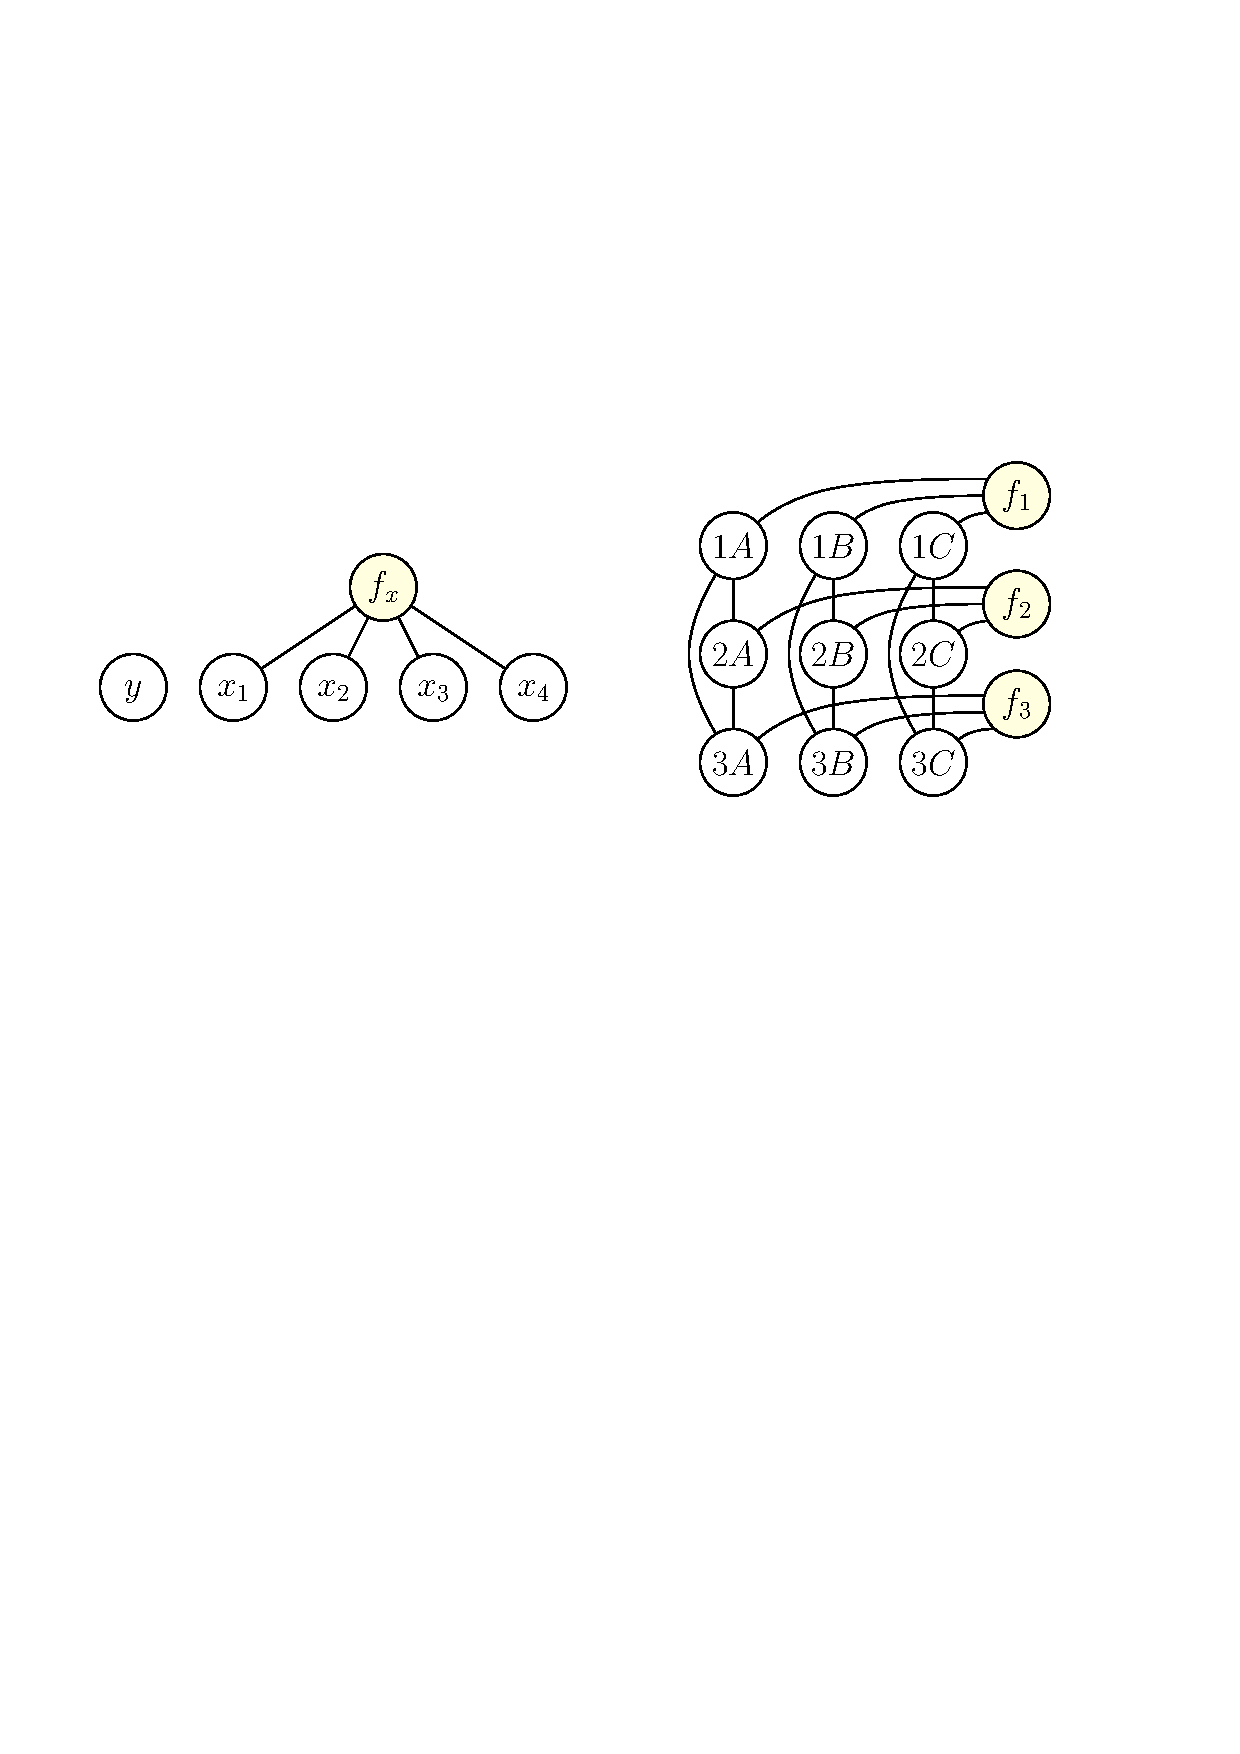
\includegraphics[width=.6\textwidth]{pictures/base-graph.pdf}
\caption{Base graph for the counterfeit coin problem with 4 coins (left) and\\
  for Mastermind with 3 pegs and 3 colours (right).}
\label{fig:base-graph}
\end{center}
\end{figure}
\end{example}

A more complicated example is the base graph of Mastermind with 3 pegs and 3 colours,
  shown on the right-hand side.
Vertices $f_1, f_2, f_3$ have separate labels, all other vertices are labelled ``variable''.
For simplicity, we leave out symbol $x$ in the figure, e.g.
  write $1A$ instead of $x_{1A}$.\eqed

\begin{lemma}\label{lma:autobase}
Let  $\perm$ be an automorphism of $B$. Then $\perm|_\Var \in\symg$.
\end{lemma}

\begin{proof}
Let $\perm$ be an automorphism of $B$ and $(t, p)$, $p=p_1,p_2,...,p_n$ an experiment.
We show that there exists a $\perm$-symmetrical experiment to $(t, p)$.

Let $F_i\subseteq F$ be a set of mapping that are present in an outcome formula
  of $t$ with parameter $\$i$.
The vertices $f(p_i)$ for $f\in F_i$ form a clique in $B$ and so must vertices
$\perm(f(p_i))$, $f\in F_i$.

Since mappings $F$ have pairwise disjoint images, two variables $x_1, x_2$
  can be connected by an edge only if there is a symbol $k\in\Sigma$ and
  mappings $f,g\in F$ such that $f(k)=x_1$, $g(k)=x_2$.

Define $r_i$ as a symbol in $\Sigma$ satisfying $f(r_i) = \perm(f(p_i))$ for some $f\in F_i$.
Note that such $r_i$ always exists because $\perm(f) = f$ for every $f\in F$.
Thanks to the aforementioned property,
  if $f(r_i) = \perm(f(p_i))$ holds
  for \emph{some} $f\in F_i$,
  it holds for \emph{all} $f\in F_i$ and the definition is thus correct.

Now, consider the experiment $(t, r)$, $r=r_1,r_2,...,r_n$.
All variables appearing directly in the parametrized formula are stabilized by $\perm$ and,
  for all expressions $f(\$i)$ it holds $f(r_i)=\perm(f(p_i))$ by the construction of $r_i$,
  which means that $(t, r)$ is $\perm$-symmetrical to $(t, p)$. \qed
\end{proof}

\subsection{Experiment graph}

Let $\form\in\Form_X$ be a formula.
An \emph{$x$-rooted tree of $\form$}
  is a graph created from the syntax tree of $\form$
  by unification of leaves that correspond to the same variables
  and adding a special vertex with label $x$ that is connected to the root
  of the syntax tree, i.e. to the top-level operator of $\form$.
Other vertices of the graph are labelled by their type (e.g. ``variable'', ``and-operator'', etc.)

In this construction, we need the trees of two formulas be isomorphic if
  and only if the formulas are syntactically equivalent.
This clearly holds if all the operators are commutative.
As the only non-commutative operator is implication, we substitute
subformulas of a form $\form -> \formx$ with $\formx \vee \neg\form$.

Let $B$ be the base graph for the given game, $\form\in\Formr$ some partial knowledge
  and $e$ an experiment.
The experiment graph $B_{\form, e}$ is constructed as follows.
\begin{itemize}
\item Begin with graph $B$.
\item Add a ``knowledge''-rooted tree of $\form$.
\item For each outcome $\formx\in\outcome(e)$, add an ``outcome''-rooted tree of $\formx$.
\end{itemize}

\begin{theorem} \label{thm:isoequiv}
If $B_{\form, e_1}$ is isomorphic to $B_{\form, e_2}$, then
 $e_1 \expeq{\form} e_2$.
\end{theorem}

\begin{proof}
Let $\permx$ be the graph isomorphism of $B_{\form, e_1}$ and $B_{\form, e_2}$ and let
  $\perm = \permx|_\Var$, considered as a permutation of $\Var$.
Since $B$ is the vertex-induced subgraph of both $B_{\form,e_1}$ and $B_{\form, e_2}$ by
  the set of vertices $\Var\cupdot F$, $\perm$ is a member of $\symg$ by \autoref{lma:autobase}.

The isomorphism $\permx$ maps the only ``knowledge''-labelled vertex in the first graph
  to the only ``knowledge''-labelled vertex in the second graph,
  which implies the equivalence of the formulas, $\form^\perm \equiv \form$.
Similarly, ``outcome''-labelled vertices are mapped to ``outcome''-labelled vertices,
  which means that $\{\formx^\perm \| \formx\in\outcome(e_1)\} = \outcome(e_2)$.
This is sufficient for the experiments to be equivalent with respect to $\form$.
  \qed
\end{proof}

\begin{example}
Recall the running example of the counterfeit coin problem with 4 coins.
Base graph for the game was shown in \autoref{ex:cc-runbase}.
Let $\form=\init\wedge\neg(x_1\vee x_2)$ be the accumulated knowledge
  of the solving process $(12, =)$ and let $e$ be experiment $3124$.
Experiment graph $B_{\form, e}$ is shown in \autoref{fig:exp-graph};
  Ex$_1$ denotes the $\exactlyk{1}$ operator.
\begin{figure}[ht]
\begin{center}
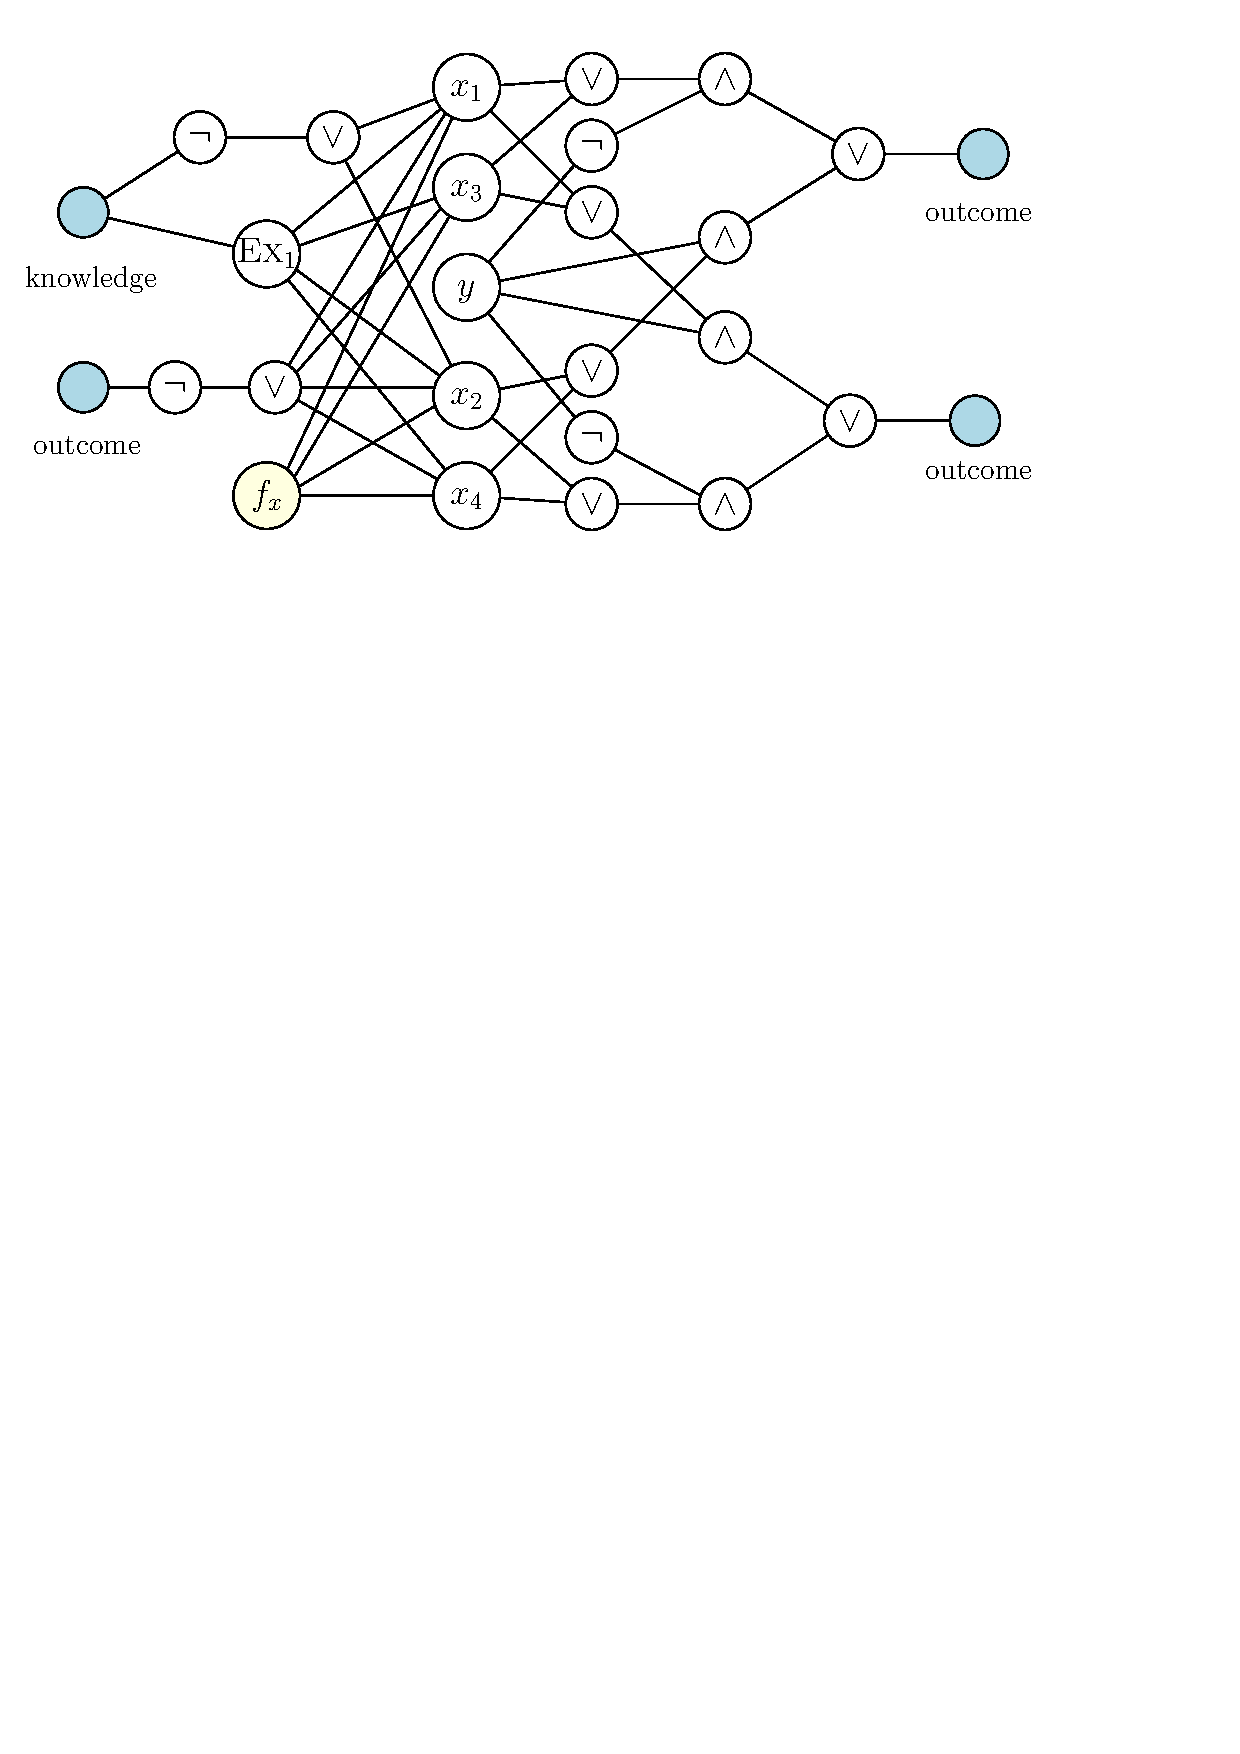
\includegraphics[width=.7\textwidth]{pictures/exp-graph.pdf}
\caption{Experiment graph for 3124 with knowledge $\init\wedge\neg(x_1\vee x_2)$.}
\label{fig:exp-graph}
\end{center}
\end{figure}

Unfortunately, the graph for experiment 43 is clearly not isomorphic to this graph,
although the experiments are equivalent with respect to $\form$.
We address this problem in the following.\eqed
\end{example}

\subsection{Improvement by fixed variables}

The previous example shows that the method explained above
  does not detect some basic equivalences.
To address the problem, we suggest the following improvement to the construction
  of $B_{\form, e}$.
\begin{enumerate}
\item Compute fixed variables of formula $\form$ using a SAT solver.
\item Simplify formula $\form$ with the knowledge of its fixed variable.
\item Simplify the outcomes of $e$, formulas $\formx\in\outcome(e)$, with
  the knowledge of fixed variables in $\form$.
\item Construct the graph as described above.
\item Label the vertices corresponding to fixed variables with ``false'' or ``true'' label,
  according to their fixed value.
\end{enumerate}

As the simplified formulas are equivalent to the original formulas,
\autoref{thm:isoequiv} also holds if the graphs $B_{\form, e_1}$, $B_{\form, e_2}$
are constructed with this approach.

\begin{example}
Let us apply the suggested improvement on the previous example.
The formula $\form = \init\wedge\neg(x_1\vee x_2)$ fixed variables
$x_1$ and $x_2$ to 0.
\autoref{fig:exp-graph-sim} shows the constructed experiment graph
  after the simplification of the formulas.

\begin{figure}[ht]
\begin{center}
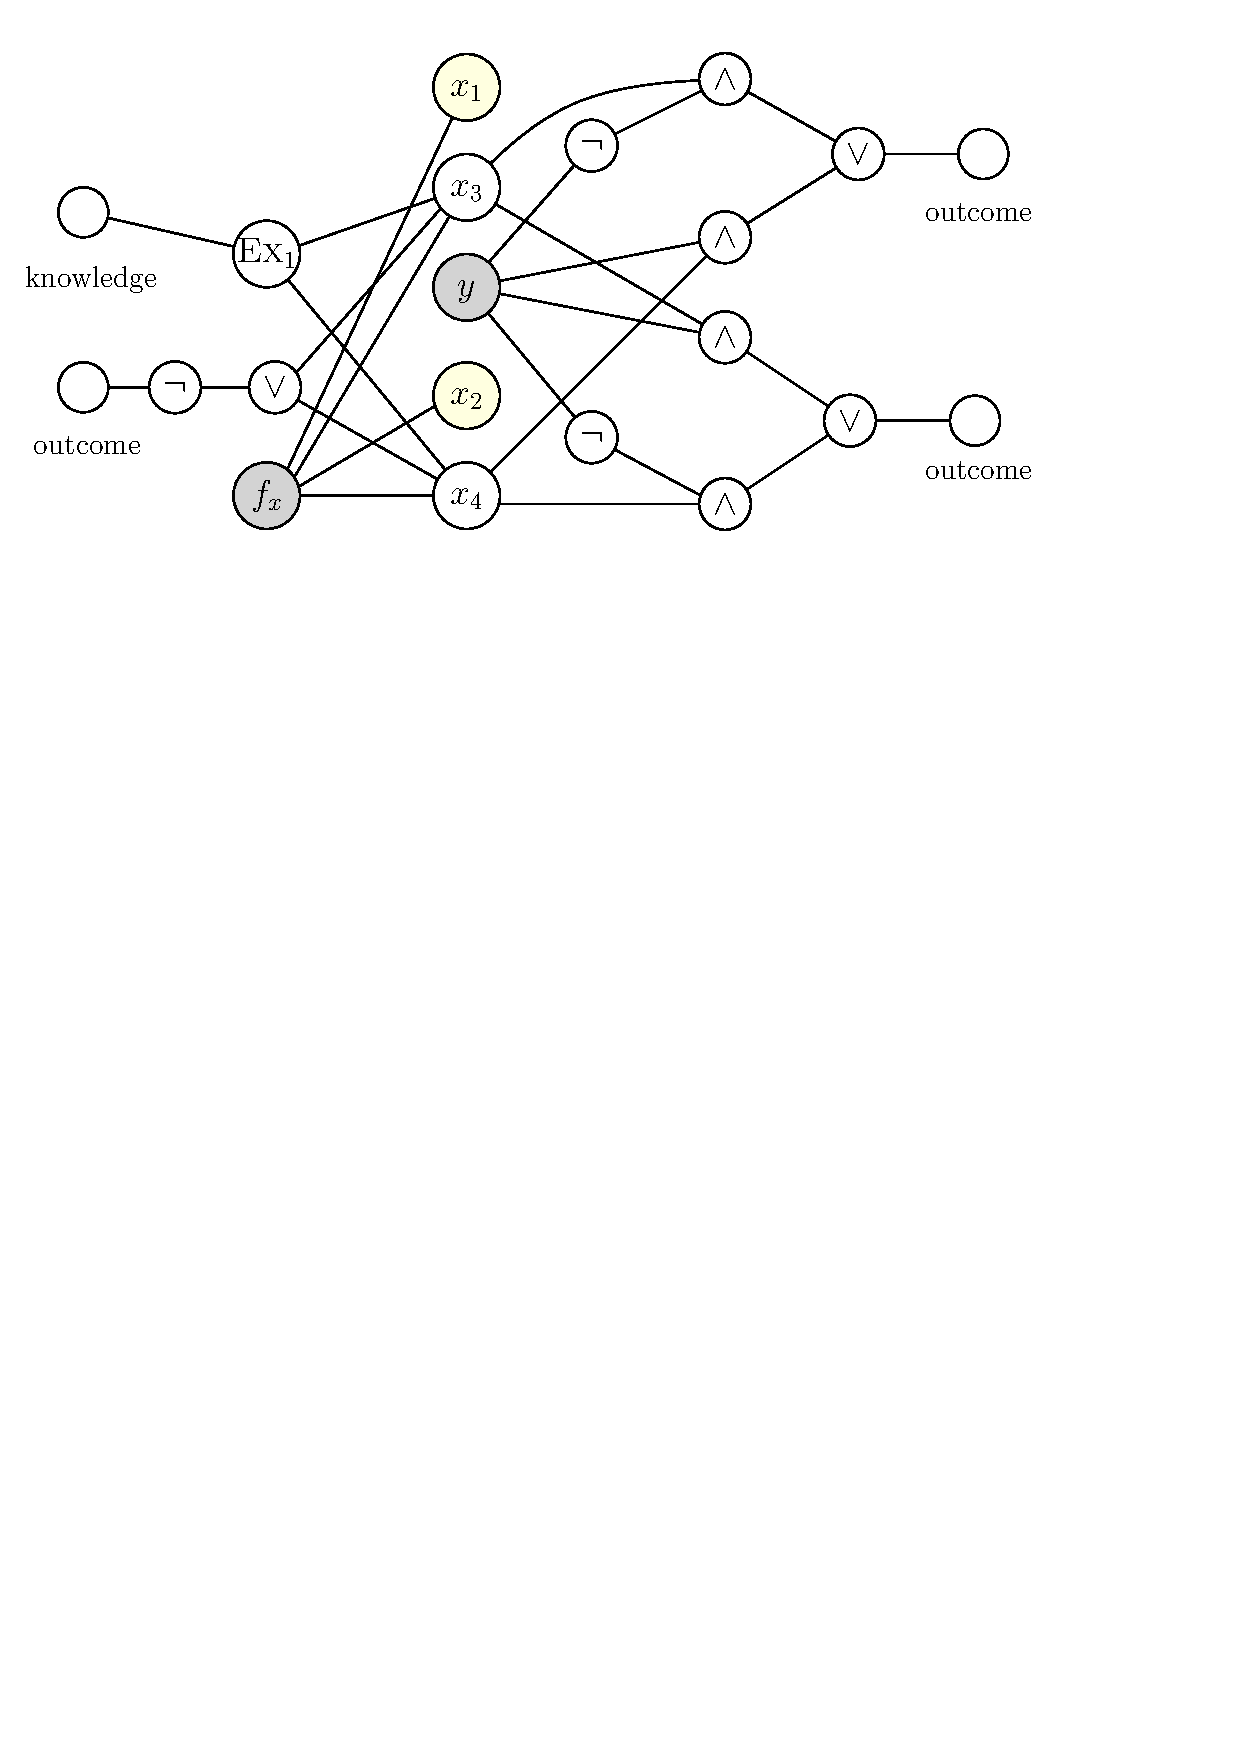
\includegraphics[width=.7\textwidth]{pictures/exp-graph-sim.pdf}
\caption{Simplified experiment graph for 3124 with knowledge $\init\wedge\neg(x_1\vee x_2)$.}
\label{fig:exp-graph-sim}
\end{center}
\end{figure}

Vertices $x_1$ and $x_2$ are now labelled ``false'' and are connected
  only to vertex $f_x$.
Compare the structure with the graph in \autoref{fig:exp-graph}.
Note that the graph is now isomorphic to the graph of experiment $43$.\eqed
\end{example}

\autoref{alg:noneqexp} describes the elimination of equivalent experiments with respect to a formula $\form$,
  which is a straightforward application of the method described in this section.
We assume we have a method to construct canonical labelling of a graph,
  which is used to decide the graph isomorphism.

\begin{algorithm}[!ht]
\caption{Elimination of equivalent experiments}
\KwIn{formula $\form$}
\KwOut{set $S\subseteq E$, such that $\forall e\in E \;\exists s \in S.\;e\expeq{\form}s$}
\label{alg:noneqexp}
\DontPrintSemicolon
$B <-$ construct the base graph for the game\;
$fixed <-$ compute fixed variables of $\form$ using a SAT solver\;
$\form' <- $ substitude values for fixed variables in $\form$ and simplify\;
Label vertices in $B$ corresponding to fixed variables with their fixed value\;
Add the ``knowledge''-rooted tree of $\form'$ to $B$\;
$S <- \emptyset$\;
$hash <- $ an empty hash table for graphs\;
\For{$e\in E$}{
  $B_e <- $ clone $B$\;
  \For{$\formx\in\outcome(e)$} {
    $\formx' <- $ substitude values for $fixed$ in $\formx$ and simplify\;
    Add ``outcome''-rooted tree of $\formx'$ to $B_e$
  }
  $B_e <- $ canonize $B_e$\;
  \If{$B_e$ is not present in $hash$}{
    $hash$.insert($B_e$)\;
    $S <- S \cup \{e\}$\;
  }
}
\Return{$S$}
\end{algorithm}

\pagebreak
\section{Well-formed check}

Experiment equivalence can be used during the verification
  that a given game is well-formed, as stated by the following lemma.

\begin{lemma} \label{lma:well-formed}
  Let $S\subseteq E$ be a subset of experiments
  such that for every $e\in E$, there exists $s\in S$
   such that $e\expeq{\init}s$.
  If the formula $\init ==> \exactlyk{1}(\outcome(e'))$ is a tautology for
  all $s\in S$, then the game is well-formed.
\end{lemma}

\begin{proof}
Assume by contradiction that the game is not well formed, i.e.
  there is $e\in E$ and $v \in \Vals$ such that the number of
  formulas in $\outcome(e)$ satisfied by $v$ is not equal to one.

If $e\in S$, the formula $\init ==> \exactlyk{1}(\outcome(e'))$ is not
  satisfied by $v$. Contradiction.

Otherwise, there exists $s\in S$ such that $e\expeq{\init}s$, i.e.
  there exists $\perm\in\Perm_\Var$ such that
$\{ \init\wedge\formx \| \formx\in\outcome(e) \} =
 \{ (\init\wedge\formx)^\perm \| \formx\in\outcome(s) \}$.
Since $\init ==> \exactlyk{1}(\outcome(s))$ is a tautology,
  the permuted formula
  $\init^\perm ==> \exactlyk{1}(\formx^\perm \| \formx\in\outcome(s))$
  is a tautology as well.
Therefore, exactly one formula from the set
 $ \{ (\init\wedge\formx)^\perm \| \formx\in\outcome(s) \}$
 is satisfiable and the same holds for
  $\{ \init\wedge\formx \| \formx\in\outcome(e) \}$,
 which implies that
 $\init ==> \exactlyk{1}(\outcome(e))$
 is a tautology. \qed
\end{proof}

\section{Analysis of one-step look-ahead strategies}

The following lemma gives us a right to disregard equivalent experiments
  during analysis of some one-step look-ahead strategies.

\begin{lemma}
Let $f: 2^\Formr ->\Rset$ be a function such that
  $f(\formset) = f(\{\form^\pi \| \form\in\formset\})$ for any
  $\formset\subseteq\Formr$ and $\pi\in\Perm_\Var$ and
  let $\eord$ be a total order of experiments $E$.
Let $\stg$ be a one-step look-ahead strategy with respect to $f$ and $\eord$, and
let $\form$ be a formula.
Suppose there are experiment $e_1$, $e_2$ such that $e_1\expeq{\form}e_2$ and $e_1\eord e_2$.
Then $\stg(\form) \not= e_2$.
\end{lemma}

\begin{proof}
If follows directly from \autoref{def:expeq} and the property of $f$ that
\[f(\{\form\wedge\formx\| \formx\in\outcome(e_1)\}) =
 f(\{\form\wedge\formx\| \formx\in\outcome(e_2)\}).\]
Since $e_1 \eord e_2$, the strategy always prefers $e_1$ to $e_2$. \qed
\end{proof}

\vspace{-5mm}
\begin{algorithm}[ht]
\caption{Analysis of a one-step look-ahead strategy}
\label{alg:stganalysis}
\DontPrintSemicolon
\KwIn{function $f: 2^\Formr -> \Rset$}
\KwOut{($w,a$), where $w$ and $a$ is the worst-case and the average-case number of experiments performed by the strategy}
$globalsum <- 0$\;
$globalmax <- 0$\;
\textsc{Analyse}($\init$, 1)\;
\Return$ (globalmax,\; globalsum \;/\; \numval\init)$\;\medskip
\setcounter{AlgoLine}{0}
\SetKwProg{optfun}{Function}{}{}
\optfun{\textsc{Analyse}\textnormal{($\form$, $depth$)}}{
$choice <- $None\;
$bestvalue <- \infty$\;
$S <- $ eliminate equivalent experiments by running \autoref{alg:noneqexp} on $\form$\;
\For{$e\in S$ (variant 1) or $e\in E$ (variant 2)}{
  $value <- f(e)$
  \If{$value < bestvalue$} {
    $choice <- e$\;
    $bestvalue <- value$\;
  }
}
\For{$\formx\in\outcome(e)$}{
  \lIf{not $\SAT{\form\wedge\formx}$}{continue}
  \eIf{$\numval(\form\wedge\formx) = 1$}{
    $globalsum <- globalsum + depth$\;
    $globalmax <- max(globalmax, depth)$\;
  }{
    \textsc{Analyse}($\form\wedge\formx$, $depth + 1$)\;
  }
}
}{}
\end{algorithm}

Note that all one-step look-ahead strategies discussed in \autoref{sec:oslas}
  satisfy the condition of the lemma.
In general, any function based on satisfiability, the number of models and/or
  the number of fixed variables of the formulas will satisfy this condition as
  these function are permutation independent.

A recursive approach for the analysis of one-step look-ahead strategies
  is shown in \autoref{alg:stganalysis}.
There are two options on line $5$ of \textsc{Analyse} function.
The first is to use the algorithm to eliminate equivalent formulas and thus
  evaluate the strategy only on a subset of experiments.
The second is to go through all possible experiments.

In general, it cannot be said which variant is faster.
This depends on the ratio between the time
  needed for graph canonization and the
  time needed for strategy evaluation.

\section{Optimal strategy synthesis}

Backtracking is the basic method for worst-case and average-case
  optimal strategy synthesis.
Our goal in this section is to prove that we can disregard
  equivalent experiments and thus significantly
  reduce branching of the algorithm in every step.

\newcommand{\optval}{\kappa}
\newcommand{\optexp}{\varepsilon}
\newcommand{\optvale}{\kappa_\textrm{exp}}
\newcommand{\optexpe}{\varepsilon_\textrm{exp}}

First, let us define $\optval(\form)$ and $\optvale(\form)$ as
 the optimal number of experiments needed to reveal the secret code
  when starting with knowledge $\form$
  in the worst-case and in the average-case, respectively.
We can say that $\optval(\form)$, resp. $\optvale(\form)$ is
  the worst-case, resp. average-case number of experiments of
  a worst-case, resp. average-case optimal strategy
  if we change the initial constraint of the game to $\form$.

Similarly, we define $\optval(\form, e)$ and $\optvale(\form, e)$ as
  the optimal number of experiment needed to reveal the secret code
  when starting with knowledge $\form$ and
  with $e$ as the first experiment.

There is an obvious relationship between $\optval(\form)$ and $\optval(\form,e)$
  and between $\optvale(\form)$ and $\optvale(\form,e)$.
For any $\form\in\Formr$,
\begin{equation}
\optval(\form) = \min_{e\in\Exp}\optval(\form, e),\textrm{ and }
\hspace{1cm}
\optvale(\form) = \min_{e\in\Exp}\optvale(\form, e).
\label{opttriv}
\end{equation}

Further, we can compute $\optval(\form, e)$ and $\optvale(\form, e)$
  from the optimal values for the subproblems after one experiment.
These relationships are based on the definitions of the worst-case
  and average-case number of experiments of a strategy
  ($\lenmax{\stg}$ and $\lenexp{\stg}$).
For any $\form\in\Formr$ and $e\in E$,
\begin{align}
\optval(\form, e) &= \left\{\begin{array}{ll}
 0 & \textrm{ if }\numval{\form} = 1, \\
 \infty & \textrm{ if }\exists\formx\in\outcome(e).\; \form\wedge\formx\equiv\form, \\
 1 + \max_{\formx\in\outcome(e)}\optval(\form\wedge\formx) &
 \textrm{ otherwise. }
\end{array}\right.\label{optval}\\
\optvale(\form, e) &= \left\{\begin{array}{ll}
 0 & \textrm{ if }\numval{\form} = 1, \\
 \infty & \textrm{ if }\exists\formx\in\outcome(e).\; \form\wedge\formx\equiv\form, \\
 1 + \frac{\sum_{\formx\in\outcome(e)}\numval{(\form\wedge\formx)}\cdot\optvale(\form\wedge\formx)}{\numval{\form}} &
 \textrm{ otherwise. }
\end{array}\right.\label{optvale}\\
\end{align}

Let us now define a set of optimal choices in a state.
For a $\form\in\Formr$, we define
\begin{align*}
\optexp(\form) &= \{ e\in E \| \forall e'\in E.\; \optval(\form, e) <= \optval(\form, e') \},\textrm{ and }\\
\optexpe(\form) &= \{ e\in E \| \forall e'\in E.\; \optvale(\form, e) <= \optvale(\form, e') \}.
\end{align*}

The following lemma is a straightforward consequence of the definitions of $\optval$ and~$\optexp$.

\begin{lemma}
Let $\stg$ be a strategy such that $\stg(\form)\in\optexp(\form)$ for every $\form\in\Formr$.
Then $\stg$ is worst-case optimal.
Similarly, let $\stg'$ be a strategy such that $\stg'(\form)\in\optexpe(\form)$ for every $\form\in\Formr$.
Then $\stg'$ is average-case optimal.
\end{lemma}

Now we are ready for the main theorem, which gives as a right to consider
  only one experiment from
  each equivalence class of $E/\expeq{\form}$
  in the state where the
  accumulated knowledge is $\form$.
The exact algorithm for optimal strategy synthesis
  with further optimizations is described in \autoref{s:cobra-modes}.

\begin{theorem}
For every $\form\in\Formr$,
\begin{enumerate}
\item $\optval(\form) = \optval(\form^\perm)$ and $\optvale(\form) = \optvale(\form^\perm)$ for all $\perm\in\symg$, and
\item if $e_1\expeq{\form} e_2$, then $e_1\in\optexp(\form) \Leftrightarrow e_2\in\optexp(\form)$ and
  $e_1\in\optexpe(\form) \Leftrightarrow e_2\in\optexpe(\form)$.
\end{enumerate}
\end{theorem}

\begin{proof}
The proof for the worst case ($\optval, \optexp$)
  and for the average-case ($\optvale, \optexpe$) is exactly the same,
  so we prove it only for worst-case.

Since $\perm\in\symg$, there exists a $\perm$-symmetrical experiment $e^\perm$
  for every $e\in E$.
Recall that $\outcome(e^\perm) = \{ \formx^\perm \| \formx\in\outcome(e)\}$.
We show by induction on the number of models of $\form$
  that $\optval(\form, \exp) = \optval(\form^\perm, \exp^\perm)$,
  which is sufficient for the first part.

As $\numval{\form} = \numval{\form^\perm}$, the statements follows directly from
  (\refeq{opttriv}) and (\refeq{optval}) for formulas with one model.
For the induction step, observe that
  $\numval(\form^\perm \wedge \formx^\perm) = \numval(\form\wedge\formx)$
  and
  $\optval(\form^\perm \wedge \formx^\perm) = \optval(\form\wedge\formx)$
  if $\form \not\equiv \form\wedge\formx$, by the induction hypothesis.
The statement now follows from (\refeq{optval})
  as the right sides are equal.

For the second part, it suffices to prove that
  $\optval(\form, e_1) = \optval(\form, e_2)$.
As the experiments are equivalent, there exists a permutation $\perm\in\symg$,
 such that
 $\{\form\wedge\formx \|\formx\in\outcome(e_1)\} =
 \{(\form\wedge\formx)^\perm \|\formx\in\outcome(e_2)\}$.
The equation now follows from (\refeq{optval}) and the facts that
 $\numval\form=\numval\form^\perm$ and $\optval(\form) = \optval(\form^\perm)$
 (proven in the first part). \qed
\end{proof}

A recursive algorithm for the computation of the value
  of an average-case optimal strategy,
  $\optvale(\form)$ is shown in \autoref{alg:acopt}.
The algorithm is based on equation (\refeq{optvale}) and
  the previous theorem.

Apart from formula $\form$, the recursive function takes another argument, $opt$,
  which is used for branch pruning.
The value of $opt$ is the best value of $\optvale(\form, e)$
  that was found so far.
Clearly, if we can be sure that $\optvale(\form, e') > opt$, we are not interested
  in the exact value as the experiment will not be selected anyway.
A lower bound on $\optvale(\form, e')$ can be computed using \autoref{lma:lbound}.

The inital value of $opt$ should be $\infty$ or an upper bound on $\optvale(\init, e)$.


\begin{algorithm}[ht]
\caption{Synthesis of average-case optimal strategy.}
\label{alg:acopt}
\DontPrintSemicolon
\SetKwProg{optfun}{Function}{}{}
\optfun{\textsc{Optimum}\textnormal{($\form$, $opt$)}}{
\lIf{$\numval{\form} = 1$}{\Return{0}}
$ lb <- \textsc{LowerBound}(\form)$\;
\lIf{$lb > opt$}{\Return{$\infty$}}
compute subset of experiments $S$ such that
  $e\in E ==> \exists e'\in S.\;e\expeq{\form}e'$\;
% $ b <- $ maximal number of satisfiable outcomes of an experiment in $S$\;
% $ lb <- \textsc{LowerBound}(\form, b)$\;
% \lIf{$lb > opt$}{\Return{$\infty$}}
\For{$s\in S$, ordered by $\max_{\formx\in\outcome(s)}\numval(\form\wedge\formx)$}
{
  \lIf{only one of $\form\wedge\formx$, $\formx\in\outcome(s)$ is satisfiable}{continue}
  $ val <- 0 $\;
  \For{$\formx\in\outcome(s)$} {
    \lIf{$\SAT{\form\wedge\formx}$}{
    $~\;\;\;\;\;val <- val + \numval(\form\wedge\formx)\cdot
      (1 + \textsc{Optimum}(\form\wedge\formx,\; opt))$}
  }
  $val <- val \;/\; \numval(\form)$\;
  \lIf{$val < opt$}{$opt <- val$}
}
\Return{$opt$}
}{}
\end{algorithm}

Note that the order of experiments on line 7
  is not necessary for correctness of the algorithm.
Our goal is to find a good experiment as soon as possible,
  because this allows us to prune many branches in the beginning.

